\section{Results} \label{sec:results}

The following section presents the findings of the study. The results are organized into qualitative results in section \ref{ssec:qual_results} and quantitative results in section \ref{ssec:quant_results}. Before presenting the results of the qualitative and quantitative analysis, the characteristics of the study participants are shortly described in section \ref{ssec:study_participants}, as well as reasons for participant exclusion.

\subsection{Study Participants} \label{ssec:study_participants}

Study participants were recruited through two channels: (1) students at the TU Dortmund recruited through chair for Enterprise Computing or personal contact and (2) colleagues of the author. A total of 20 participants were invited to participate throughout July 2025. The experiment was conducted in August 2025 with 13 of the participants, while 2 participants were dropped from the study due to time constraints. One participant was excluded from the analysis due to not following the instructions for the think aloud protocols sufficiently, producing unusable data. The selection process is summarized in Figure \ref{fig:participant_flow}.

\begin{figure}[ht]
    \centering
    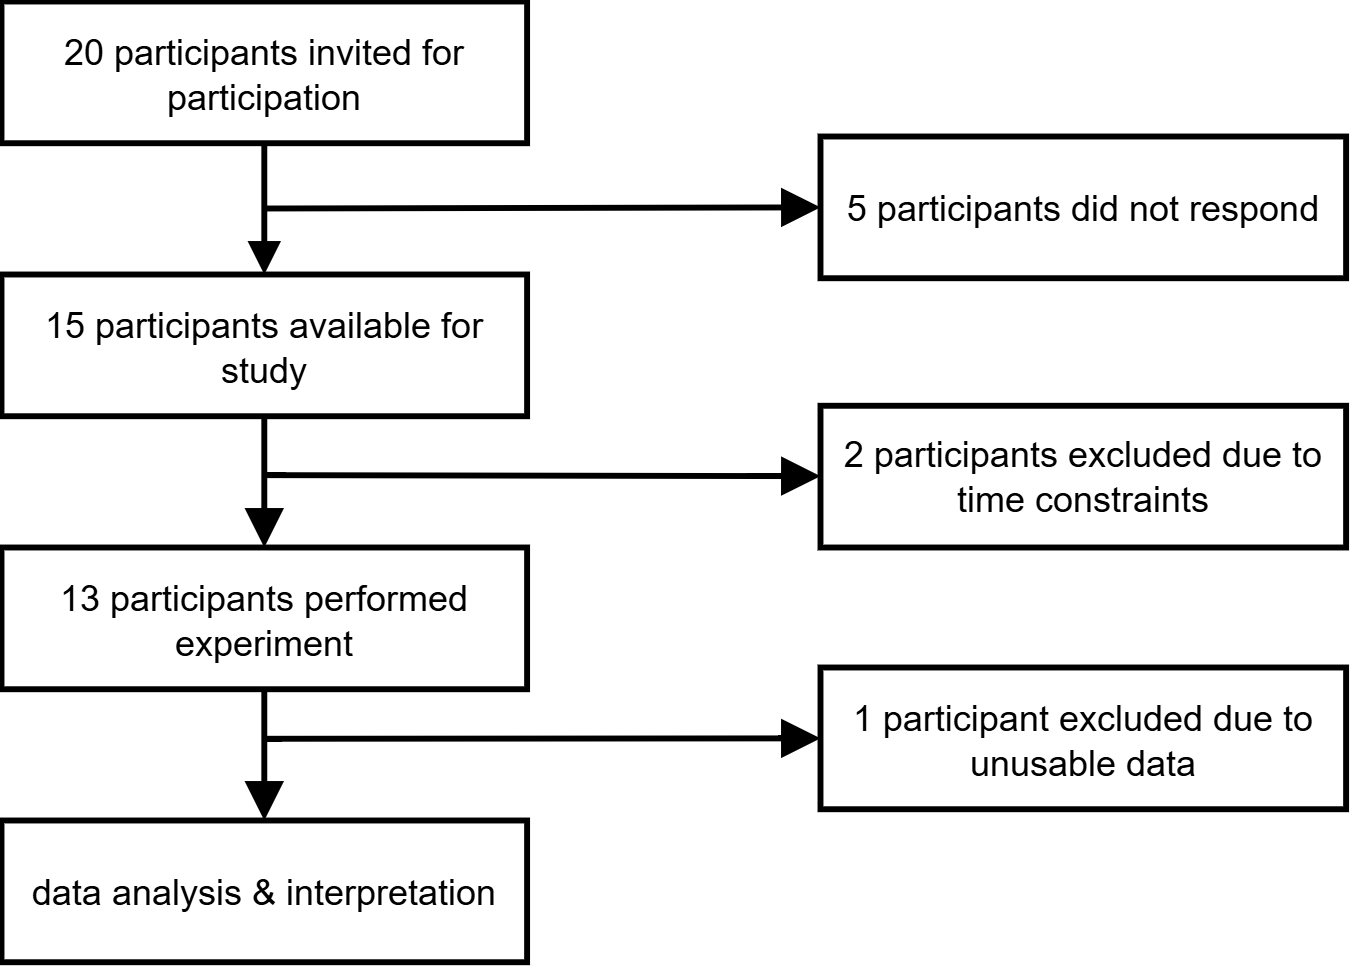
\includegraphics[width=0.5\textwidth]{images/fig-participant_flowchart.png}
    \caption{Participant Selection Flowchart}
    \label{fig:participant_flow}
\end{figure}

The participants were exclusively male, with additional demographic information about age and education presented in Table \ref{tab:age_dist} and Table \ref{tab:edu_bg}. The final sample consisted of 12 participants, with 5 in group (B) without explanations and 7 in group (E) with explanations.

\begingroup
\tablespacing

\begin{table}[ht]
    \parbox{.45\linewidth}{
        \centering
        \begin{tabular}{cc}
            Age Range & Count \\
            \hline
            20--29 & 8 \\
            30--39 & 2 \\
            40--49 & 1 \\
            60--69 & 1
        \end{tabular}
        \caption{Age Distribution of Participants}
        \label{tab:age_dist}
    }
    \hfill
    \parbox{.45\linewidth}{
        \begin{tabular}{cc}
            Education Level & Count \\
            \hline
            University Degree & 8 \\
            Vocational Training & 2 \\
            Grammar School & 2
        \end{tabular}
        \caption{Educational Background of Participants}
        \label{tab:edu_bg}
    }
\end{table}

\endgroup

\subsection{Qualitative Results} \label{ssec:qual_results}

The qualitative data collected from the think-aloud protocols was analysed as described in section \ref{sssec:qualitative_analysis}. The codes produced in the first round of coding, were then grouped into categories (axes). The four main conclusions drawn from the qualitative data are presented in the following sections: Usage patterns (\ref{sssec:usage_patterns}), errors and conflicts (\ref{sssec:errors_conflicts}), reflection and learning (\ref{sssec:reflection_learning}) and explanation usage (\ref{sssec:explanation_usage}).

\subsubsection{Usage Patterns} \label{sssec:usage_patterns}

Participants in both groups utilized the chatbot for varying purposes, if they decided to use it at all. Questions posed to the chatbot ranged from very specific questions for formulas to more general questions asking for a solution approach. Some participants used the chatbot to verify their own solutions or solution approaches. Taking into account the possibility of non-use of the chatbot, four different usage patterns can be identified, which are presented in Table \ref{tab:usage_patterns}.

\begin{ctable}
    \begin{tabularx}{\textwidth}{l|X|X}
        \textbf{Usage Pattern} & \textbf{Definition} & \textbf{Example} \\
        \hline
        Non-Use & The participant does not use the chatbot at all & “I did not need the LLM for that.” (P3) \\
        Fact Questions & The participant uses the chatbot to ask for specific facts, formulas, or definitions & “What is the formula for the circumference of a circle if 'r' is given?” (P13) \\
        Approach Questions & The participant uses the chatbot to ask for a solution or solution approach & “What approach should I take and how should I take the ratio into account.” (P4) \\
        Validation Questions & The participant uses the chatbot to verify their own solution or solution approach & “I'll send the solution to [\dots] the chatbot to see if it makes sense.” (P5)
    \end{tabularx}
    \caption{Usage Patterns of the Chatbot}
    \label{tab:usage_patterns}
\end{ctable}

The usage pattern of \textit{Non-Use} is noteworthy, as the decision to not use the chatbot was only commented by two participants (P3, P8) after the fact. Other participants also solved tasks without using the chatbot, but did not mention this decision at all. This indicates that the decision whether to use the chatbot or not, is not a conscious decision, but rather a subconscious one. Additionally, the usage patterns could change during the same task, with participants starting with approach questions (for an initial hint) and later switching to validation questions, indicating that a (subconscious) decision is made for each interaction with the chatbot.

Overall the usage patterns align with the behaviour for cognitive offloading described in section \ref{sssec:cognitive_offloading}. This particularly applies to the decision whether and how to use the chatbot, which is “[\dots] influenced by a metacognitive evaluation of the available options” \parencite{Risko2015}. A factor that could influence these decisions is the perceived difficulty of the task, which was mentioned by several participants prior to using the chatbot (P1, P5). Based on the behaviour of participants combined with the think-aloud protocols, it can also be assumed, that the \textit{Availability} heuristic \parencite{Tversky1974} played a role in the decision whether to use the chatbot or not. Participants more often used the chatbot for developing a solution approach, if they had exhausted their own ideas (P3, P8, P10). A third factor that could influence these decisions is the perceived effort of using the chatbot compared to solving the task without it. This is supported by the fact that some participants justified their use of the chatbot by stating they did not “want to [solve the problem]” themselves (P5).

\subsubsection{Errors and Conflicts} \label{sssec:errors_conflicts}

Participants in both groups encountered errors and conflicts during their interactions with the chatbot. It is important to note, that the problems described here, are conflicts and errors perceived by the participants. They can be caused by either the chatbot or the participant. These perceived issues can be grouped into two categories, which are presented in Table \ref{tab:conflicts_errors}.

\begin{ctable}
    \begin{tabularx}{\textwidth}{l|X|X}
        \textbf{Category} & \textbf{Definition} & \textbf{Example} \\
        \hline
        Incorrect Information & The chatbot provides factually incorrect information & “But it [the chatbot] says, that I have $\overline{AB}$ given, which is not correct either.” (P4) \\
        Conflicting Information & The chatbot provides information that contradicts previous responses or known facts & “First it [the chatbot] says 'almost correct', then 'correct' [for the same solution]” (P11) \\
    \end{tabularx}
    \caption{Categories of Errors and Conflicts with the Chatbot}
    \label{tab:conflicts_errors}
\end{ctable}

The most frequently encountered issue was \textit{incorrect information}, where participants perceived the chatbot's responses as factually incorrect (P4, P8, P13, P15). In many cases however, the participants simply misread the response (P8) or forgot information provided in the task or previously calculated (P4, P13, P15). In a similar fashion participants misunderstood or misinterpreted the chatbot's response (e.g. P11, P13). Conversely, during task 54 participants frequently received wrong advice from the chatbot, but did not recognize the error immediately. Given that none mentioned the wrong information from the chatbot in their think-aloud protocols, it can be assumed that a form of “satisficing” \parencite{Simon1955} took place, where participants accepted the chatbot's response without further scrutiny.

The conflict behaviour observed during the study aligns with the findings from \textcite{Jussupow2021}, where medical practitioners experienced similar conflicts when using a decision support system to diagnose \ac{COPD}. When being confronted with AI decisions that conflicted with their own assessment, the practitioners experience a belief conflict, where they had to decide whether to trust their own judgement or the AI's decision. A similar conflict was observed in this study, but participants did rarely verbalize the conflict. Instead, most participants moved to the validation conflict, seeking additional information to resolve the conflict. “Aiming to resolve the validation conflict, decision makers continuously evaluate their personal confidence into their own frame against their perception of the system accuracy” \parencite{Jussupow2021}. For these purposes participants employed strategies similar to those described by \textcite{Jussupow2021}, such as seeking additional information to confirm either position (self-monitoring or system monitoring). Additionally, participants sometimes decided to correct the chatbot with additional prompts, effectively taking on the role of a teacher (teaching the system). During the study the validation conflict was often resolved users discovering their own mistakes (P4, P9, P15) and adopting the chatbot's position.

Participants sometimes struggled to resolve conflicts especially if they reached the stage of the validation conflict. Participant 5, for example, stated “I do not know where the [problem] is right now.” after struggling to understand a solution approach suggested by the chatbot. This aligns with the findings of \textcite{Jussupow2021}, who observed that users struggle to appropriately switch from type 1 to type 2 cognition when confronted with conflicting AI advice. This is underlined by participant 2 stating, “It is hard sometimes to connect [the chatbot's responses] to what I am thinking” after having completed all tasks.

\subsubsection{Reflection and Learning} \label{sssec:reflection_learning}

The think-aloud protocols also showed, that participants did not actively reflect on every interaction with the chatbot. Reflection primarily occurred after participants resolved a conflict with the chatbot (P8, P11) or when they were positively surprised by the chatbot's assistance (P1, P2). Participant 8 noted that it was “sad, that the chatbot does not detect these logic errors” after realizing he had made a mistake transforming a formula step by step. On the other hand, participant 1 assessed, that “the chatbot helped quite a lot”. It is unclear under which conditions participants actively reflect on interaction with the chatbot, but two general cognitive patterns may play a role:

\begin{itemize}
    \item \textbf{Abnormality:} The fact, that participants only reflected on interactions that were either very positive or negative, could be explained through the abnormality that these scenarios represent. Humans tend to focus on events perceived as abnormal or unexpected, when seeking and constructing explanations \parencite{Miller2019}.
    \item \textbf{Anchoring \& Adjustment:} The heuristic of anchoring and adjustment \parencite{Tversky1974} relates to the notion of abnormality as well. Participants could have anchored their expectations of the chatbot's performance based on prior experiences with chatbots or AI systems in general. When the chatbot's performance deviated significantly from these expectations, it could have triggered reflection.
\end{itemize}

Some interactions with the chatbot also led to learning effects, where participants adapted their interaction strategy based on previous experiences. For example participant 8 encountered an issue, where the chatbot was unable to follow multiple changes to a formula in a single message. After this incident, the participant reflected that “the AI could not cope with the fact I calculated the squares” and subsequently adapted his interaction strategy to send smaller, incremental changes to the chatbot. Since questionnaires were only administered after all tasks were completed, no quantitative data about the evolution of the participants' perceptions is available.

\subsubsection{Explanation Usage} \label{sssec:explanation_usage}

Participants rarely actively engaged with the explanations provided by the chatbot in group (E). Only two participants (P8, P9) explicitly mention the \ac{CoT} explanation. In both instances the explanation was treated as additional information, that was used once the user was stuck. Other participants in group (E) did not mention the explanations at all. Similarly, users in group (B) did not comment on the lack of explanations.
% Clean up this setence to aviod interpreting
Therefore, the explanations did not seem to have a significant impact on the participants' behaviour or perception of the chatbot. The instances where the explanations were used, could also be due to the interface design, which initially hid the explanations in a collapsed section.

\subsubsection{Anthropomorphism} \label{sssec:anthropomorphism}

Several participants anthropomorphized the chatbot, attributing human-like characteristics to it. Several participants actively thanked the chatbot, when receiving help or a satisfactory response (P2, P11). Additionally, participants often referred to the chatbot as “he” or “it” and referring to their exchanges using terminology often used for human conversation (e.g. “I'll ask the chatbot”, “The chatbot says [\dots]”). This anthropomorphism could have influenced the participants' perceptions of the chatbot's capabilities and trustworthiness \parencite{Li2022}.

\subsection{Quantitative Results} \label{ssec:quant_results}

The quantitative data collected from the questionnaires was cleaned and analysed as described in section \ref{sssec:quantitative_analysis}. The quantitative analysis focuses on the differences between the two groups ((E) with explanations and (B) without explanations as baseline).
For readability results will be rounded to three decimals.

\subsubsection{Evaluation Procedure} \label{sssec:eval_procedure}

In total seven constructs were evaluated using established questionnaires, as described in section \ref{sssec:quantitative_analysis}. The raw data was prepared by excluding participants that did not follow the instructions sufficiently (see section \ref{ssec:study_participants}) and calculating the mean score for each construct. The mean scores were then compared between the two groups using Mann-Whitney U tests. The results of the quantitative evaluation are presented in Table \ref{tab:quant_results}. The table shows the mean scores for each construct split by Group, as well as the U statistic and p-value for the Mann-Whitney U tests. A significance level of $\alpha = 0.1$ was used for all tests.

% TODO: Create a legend for the table?

\begin{ctable}
    \begin{tabularx}{\textwidth}{l|X|X|X|X|X}
        \textbf{Construct} & \textbf{Mean (B)} & \textbf{Mean (E)} & \textbf{U} & \textbf{p-value} \\
        \hline
        Perceived Usefulness $\uparrow$ & $5.233$ &  $5.905$ &  $9.000$ &  $0.095$* \\
        Perceived Ease of Use $\uparrow$ & $6.300$ &  $5.929$ &  $21.000$ &  $0.745$ \\
        Computer Self-Efficacy $\uparrow$ & $9.240$ &  $8.214$ &  $19.500$ &  $0.659$ \\
        Mental Load $\downarrow$ & $12.800$ &  $10.714$ &  $21.500$ &  $0.282$ \\
        Performance $\downarrow$ & $8.000$ &  $3.857$ &  $24.500$ &  $0.143$ \\
        Effort $\downarrow$ & $10.800$ &  $9.429$ &  $18.000$ &  $0.500$ \\
        Frustration $\downarrow$ & $12.200$ &  $2.571$ &  $33.500$ &  $0.005$* \\
    \end{tabularx}
    \caption[Quantitative Results of the Study]{Quantitative Results of the Study. Arrows indicate if a higher or lower score is better. Constructs marked with * are significant.}
    \label{tab:quant_results}
\end{ctable}

The results indicate, that the initial hypotheses that explanations improve acceptance and reduce load and stress are correct. The constructs \textit{perceived usefulness} and \textit{frustration} show statistically significant differences between the two groups. Even though the other constructs do not show statistically significant differences, the scores indicate, that explanations could have a positive effect on these constructs as well. The two statistically significant constructs are discussed further in the following sections.

Further statistical analysis (e.g. correlation of constructs) has been omitted due to the small sample size. Additional information about the quantitative evaluation can be found in the repository accompanying this thesis \parencite{Goepfert2025}. This includes the raw data, as well as the analysis scripts used to prepare, analyse and visualize the data. The analysis scripts are written in Python as Jupyter Notebooks and rely on Pandas, SciPy and Matplotlib.

\subsubsection{Perceived Usefulness} \label{sssec:model_acceptance}

The \textit{perceived usefulness} of the chatbot was significantly higher in group (E) with explanations ($M=5.905$) compared to group (B) without explanations ($M=5.233$) with $p=0.095$ ($U=9.000$). This indicates, that participants in group (E) found the chatbot more useful for completing the tasks compared to participants in group (B). While, the perceived ease of use did not differ significantly between the two groups, the scores still indicate an increased acceptance of the chatbot with explanations. The limited differences in perceived ease of use can be explained by the fact, that the models were identical in all terms except for the system prompt and the response structure. Therefore, the interaction with the chatbot was similar in both groups, leading to similar ease of use perceptions.

The difference in response structure could be a factor influencing the perceived usefulness. The structure of the responses in group (E) lead to shorter and more concise answers when the explanations were collapsed. Participant 4 (B) noted he was given “too much response” by the chatbot. The reduced verbosity in group (E) could have led to a perception of increased usefulness, as participants were able to quickly extract the relevant information from the chatbot's responses. Conversely, the explanations were used as additional information when participants were stuck (see Section \ref{sssec:explanation_usage}). This could have led to a perception of increased usefulness, as participants were able to get additional help when needed.

% this implies a potential underlying benefit of explanations, which is inducing a more structured response format, that in of itself could be beneficial

\subsubsection{Frustration} \label{sssec:frustration}

Group (E) experienced significantly less \textit{frustration} ($M=2.571$) compared to group (B) ($M=12.200$), with $p=0.005$ ($U=33.500$). This indicates, that participants in group (E) felt less frustrated when using the chatbot compared to participants in group (B). The reduced frustration could be due to several factors. Similar to the perceived usefulness, the structured response format could have played a role. The shortened responses made it easier for participants to extract relevant information, leading to reduced \textit{cognitive load} and \textit{effort}. This is supported by the lower scores for \textit{mental load} and \textit{effort} in group (E), even though these differences were not statistically significant. Additionally, the presence of explanations could have provided participants with a sense of transparency and understanding of the chatbot's reasoning process. Even though the explanations were rarely used, their mere presence could have reduced uncertainty and increased trust in the chatbot's responses, leading to reduced frustration.

% This is a little thin and I could check what additional info I can put in here (later)
